\documentclass{article}

\usepackage{amsmath}
\usepackage{graphicx}
\usepackage{subfig}
\usepackage{float}
\usepackage{hyperref}

\title{Applying Regression Test Selection on the example of Business Central}
\author{Diego Joshua Martinez Pineda (diem@itu.dk)\\Supervisor: Mahsa Varshosaz (mahv@itu.dk)}

\begin{document}
\maketitle

\begin{abstract}
In this research project, we address the problem of implementing a test selection algorithm on the Business Central project. For the scope of this project, a single test selection algorithm was implemented, which is based on test coverage information. The findings of this work should serve as a foundation to explore the different selection and prioritization techniques in this system. Much of the work presented here is invested into understanding the context and setting of the system, sufficiently to execute the algorithm in actual revision examples. The insights acquired provide a basis for future evaluation settings to increase the validity of the results and implementation of future algorithms to be evaluated.
\end{abstract}

\section{Introduction}\label{section:overview}
   When working with large software systems, regression testing is a valuable technique that increases the confidence of the product stakeholders that future revisions, new features, and evolution of the system will not break previous functionality.

   For this reason, it is common for products to have the execution of the regression test suite as part of the main pipeline of the product. However, when systems are sufficiently large, it becomes very expensive to run the full suite of tests.

   A test selection algorithm aims at choosing a subset of a full test suite to run, that is not as expensive as running all tests cases. However, this selection must preserve the capabilities of fault detection that the full test suite has. Tests must be selected carefully so that the confidence in fault detection is not lost due to running only a subset of tests.

   The problem of test selection has been very active in the research community, it is widely studied and several implementations on industrial software exist. Surveys and literature reviews have been conducted, later in section \ref{section:alg-and-context} we expand on a survey by Yoo et. al. \cite{Yoo2009RegressionTM} and another from Pan et. al. \cite{Pan2021TestCS}.

   Business Central is an Enterprise Resource Planning software (ERP) from Microsoft, which is a large software system, with different sets of test suites for the diverse aspects of the product.

   In this project, the selection of a subset of the test suite of the application code (business logic) is explored. 

   We aim to explore different test selection techniques for this system, to reduce the time and computing power required to detect faults in the current CI pipeline. The pipeline is triggered several times per day on the regular development cycle of the product, our aim is to improve its execution.

   The business logic of the system is written on AL, a DSL similar to Pascal that has primitives for interacting with the runtime of Business Central.

The idea for the method explored in this research project is to use the line coverage information that each test case produces. By looking at which lines were modified on a given change, we extract and exploit the information about which tests were covering those particular lines for selecting tests.

For example, see figure \ref{fig:diff}. Here we can see a \texttt{diff} of an AL code file on a given revision that added lines in between what previously were lines 30-31, and 39-40. Also what was previously line 29 was removed. Therefore, provided that we know which tests were hitting those lines, then we could propose them as a part of the tests to be selected.

\begin{figure}[H]
  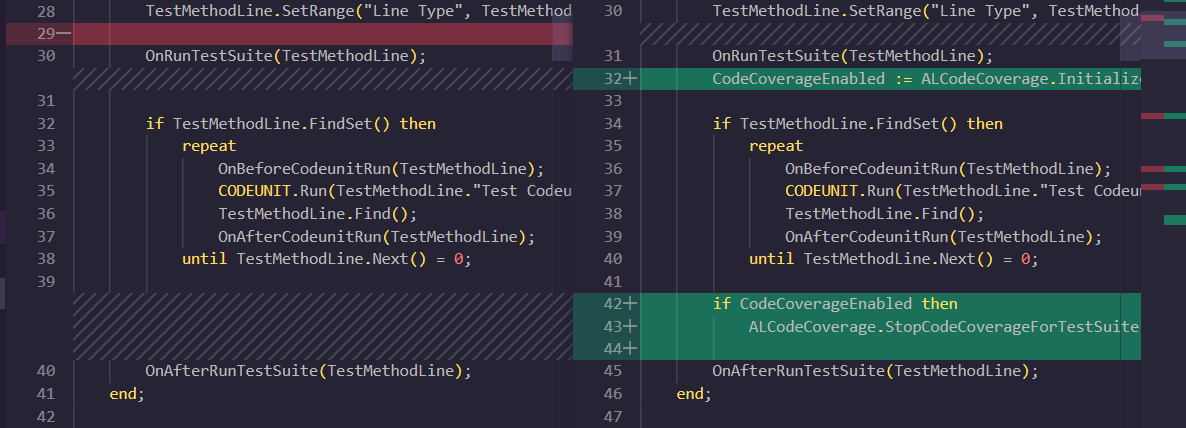
\includegraphics[width=\textwidth]{images/diff.png}
  \caption{A revision change on AL code.}
  \label{fig:diff}
\end{figure}

Intuitively, this can be a suitable heuristic to select tests. However, we do not claim it is sufficient, further examples can show that this heuristic fails in some cases. For example, when a part of the code is dependent on the side-effects it produces; then changing the environment through the side-effects of a revision, can cause a seemingly unrelated set of test cases to fail.

This method is meant to provide a foundation for further explorations on selection methods using different criteria besides this straightforward heuristic. In this project, we implemented this technique, along with the infrastructure required to evaluate it on Business Central. We compared similar techniques found in the literature, while also describing the different ways we can extend this method.

\section{Background}\label{section:al-background-info}
Before explaining details of the work, we present for reference and clarity a minimal background knowledge required to understand how code and tests in AL are defined.

As mentioned in the introduction, AL is a DSL for Business Central and extensions for this system. The code is organized in several \emph{AL objects}, which do not resemble objects in the traditional OOP sense, but objects from the system's runtime. \emph{AL objects} have different types, for example:
\begin{itemize}
\item \emph{Tables}. Corresponding to underlying SQL Server tables.
\item \emph{Pages}. Corresponding to interactive pages the user can see.
\item \emph{Codeunits}. Modules with \emph{procedures}, that is code that can be reused throughout the codebase
\end{itemize}

Each AL file in the codebase has as part of its definition, its type of object, and a numeric ID. Such a pair must be unique for a given codebase.

To make things more concrete, figure \ref{fig:al-examples} shows an example of AL objects of types \emph{page} and \emph{table}. They are identified by both the type of object and ID, notice in this example, they share the same id: 5200, but they differ on the type of object.
\begin{figure}[H]
  \centering
  \subfloat[\centering AL Page]{{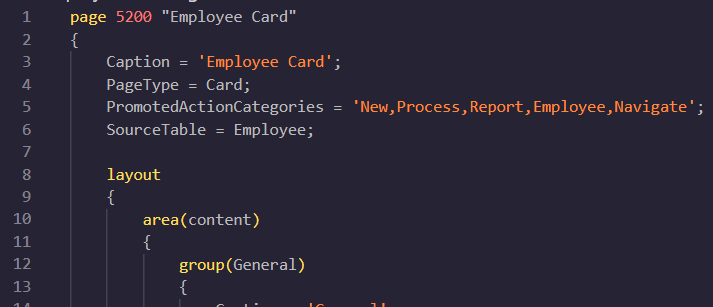
\includegraphics[width=5.5cm]{images/alpage.png} }}
  \qquad
  \subfloat[\centering AL Table]{{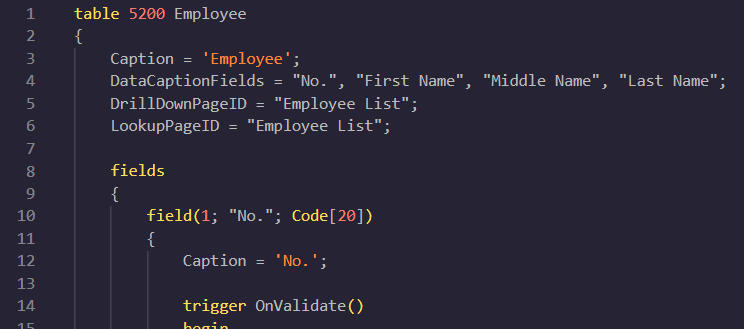
\includegraphics[width=5.5cm]{images/altable.png} }}
  \caption{Examples of \emph{AL Objects}. }
  \label{fig:al-examples}
\end{figure}

A mechanism for code reuse in this language is, as listed above, \emph{codeunits}, which is similar to the concept of ``modules'' in other languages. They consist of several \emph{procedures}. See an example in figure \ref{fig:codeunit-example}. Procedures defined on \emph{codeunit}s can be called from any other object in the codebase.
\begin{figure}[H]
  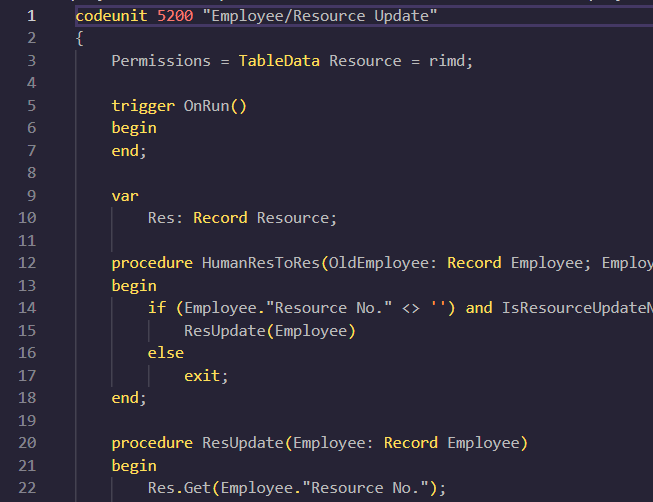
\includegraphics[width=\textwidth]{images/alcodeunit.png}
  \caption{Example of an \emph{AL Codeunit} with procedures \texttt{HumanResToRes} and \texttt{ResUpdate}.}
  \label{fig:codeunit-example}
\end{figure}

Finally, we explain how test scenarios for AL code are defined. Unit and scenario tests for application code are written in AL as well. They correspond to \emph{codeunits} that are marked as tests. Procedures within such a \emph{test codeunit} may correspond to scenarios to be tested. See figure \ref{fig:al-test-examples} for a typical example on how \emph{codeunits} are marked as tests and a scenario example. In the example, we see that the keyword \texttt{Subtype} is used to define the \emph{codeunit} as a \emph{test codeunit}. We can see a test scenario defined as a procedure on this \emph{codeunit} called \texttt{TestVATStatementReportLineMissing}. A typical test would describe in comments the scenario being tested as shown in the figure.

\begin{figure}[H]
  \centering
  \subfloat[\centering AL Test Codeunit Definition]{{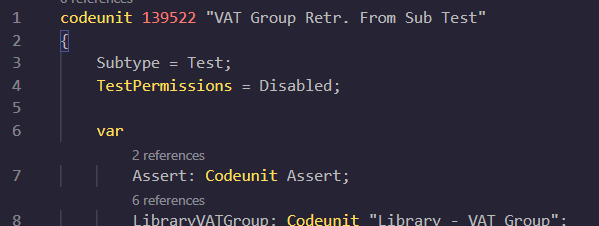
\includegraphics[width=5.5cm]{images/altestcodeunit.png} }}
  \qquad
  \subfloat[\centering AL Test Procedure - Scenario]{{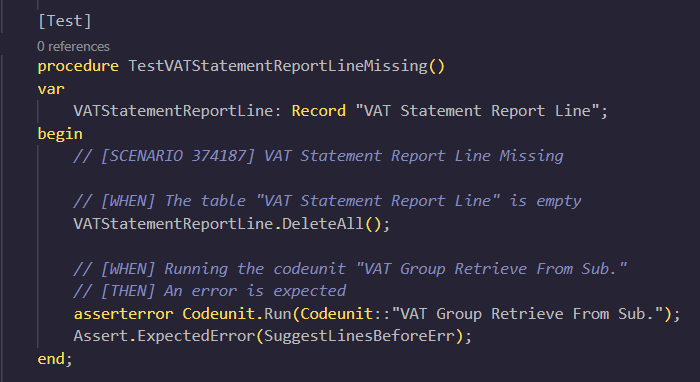
\includegraphics[width=5.5cm]{images/altestscenario.png} }}
  \caption{Examples of definition of AL Test Scenarios. }
  \label{fig:al-test-examples}
\end{figure}


\section{Test Selection Method}
\subsection{Coverage information of test runs on AL}\label{section:cov-info}
AL provides primitives to dynamically record line coverage information when executing arbitrary sections of code. This line coverage information has the following components, relevant for the selection method:
\begin{itemize}
\item Object ID
\item Object type
\item Line number
\item Number of hits
\end{itemize}

As explained in the previous section, both the \emph{Object ID} and \emph{Object Type} identify a file in the codebase. The \emph{Number of hits} counts how many times the \emph{Line number} of that file was recorded.

It is relevant to stress that this information does not provide a file path on the codebase directly, but only a mean for identification.

Currently on the system, this primitive is used throughout the execution of the test suite. These measures test coverage information, providing the set of objects and lines covered by the suite, and it is used to impose coverage requirements for new additions to the codebase.

This means, that the information obtained by recording coverage throughout the complete execution of the test suite, cannot be used to distinguish coverage information between different test scenarios. The coverage information currently available on the pipeline of the system does not have information about which lines were hit by a particular test, but it only determines that it was hit by some test on the test suite.

However, previously in section \ref{section:overview}, we described the method as selecting those test cases which covered a particular set of lines. With the current test coverage information, it is not possible to make that distinction.

For this reason, we need changes on the test runner, to allow for individual tracking of coverage information per test case. However, these changes are currently not on the main pipeline of the product\footnote{These changes were not the work of the author but from Nikola Kukrika nikolak@microsoft.com}. The coverage information it provides cannot be obtained from the CI pipeline of the system.

Another relevant technical consideration of how this information was dealt with, is how the output of the coverage information of each test case was stored. The modified test runner outputs a set of CSV files, one corresponding for each test procedure, containing the described coverage information together with the contents of the covered line.

As a part of the work for this project, a different organization of this information was proposed and implemented. To allow for efficient querying of information in different ways, we proposed an SQLite database. A parsing-loading program was developed for this purpose. This provides a better organization for dealing with the information since the database is a single file. The reason for proposing a file database instead of a regular database is that coverage information can also be used for different purposes and easy distribution was desired.

Figure \ref{fig:erdiagram} shows the ER diagram in crow's foot notation of the DB schema proposed. AL Objects are modeled with their lines in a one-to-many relationship. These in turn are joined through the \texttt{coverage data} pivot table with the test procedures.
\begin{figure}[H]
  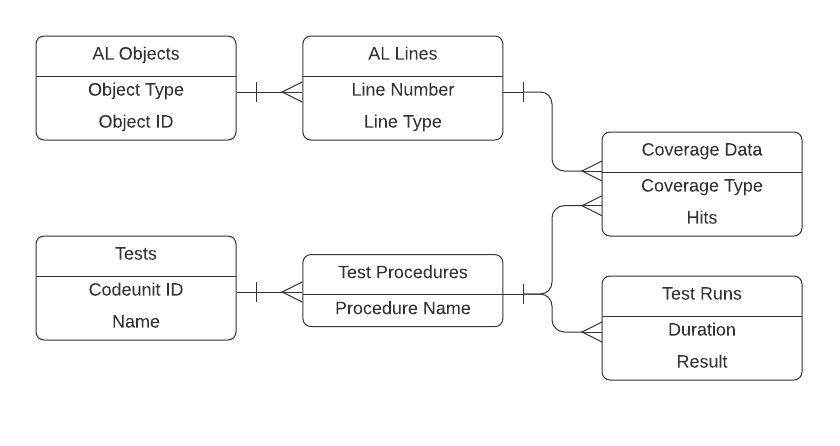
\includegraphics[width=\textwidth]{images/erdiagram.png}
  \caption{ER diagram for the proposed coverage database schema}\label{fig:erdiagram}
\end{figure}

\subsection{Representing revision differences}\label{section:rev-diffs}

The codebase with the business logic is composed of several AL applications.

When working on a new revision, some of the files on these applications are changed, removed, or added. To represent the changes done on a set of text files, it is common to use \texttt{diff}s.

The output information of such \texttt{diff} is the set of file paths added, removed, or changed, together with the lines where these changes occurred.

However, in the previous section, we explained that the coverage information we can extract includes the Object Id and Object Type where line coverage was recorded. While these properties correspond uniquely to a file in the codebase, directly checking the file path where the code was changed does not lead to getting the Object Id and Object Type that the file has.

Furthermore, we are considering changes on the whole codebase, that may imply changes on tests as well. For example, adding new test procedures. For these kinds of changes, it is not desirable to have the same interpretation on tests that should be selected. Whenever test procedures are added, they should be at least selected. This would not be possible by only restricting criteria for test case selection to coverage information since these tests did not exist previously.

These two situations show that more information than just the file path and lines changed is required from a given revision change. For this selection method, a lightweight parsing was performed on the given changed files to extract which Object Id is changed, and whether or not such object is a \emph{test codeunit}.

Notice that the choice of what information to extract from a given revision change was just to address these two situations. We could however extract more information, enhancing our knowledge of changes caused by the revision. This could be even more granular, for example, to detect changes on specific procedures, addition of procedures, definition of new columns on a table. In general, semantical information related to changes. This could be a direction for future work, as input for more complex selection criteria (See section \ref{section:future-work}). Currently, only a simple representation is used since it suffices for our method. Also, it would require more complex parsing procedures.

For completeness, table \ref{table:revision-changes} shows the information extracted for identifying a set of revision changes. See for example how we represent the change of adding lines to an AL object, we identify it as a change of type \texttt{AddLinesObject}, and we store the \texttt{objectId} of the object changed and \texttt{afterLine} is the number after which the new lines were appended (as the number it had in the original revision).

\begin{table}[H]
\centering
\begin{tabular}{||c c||} 
 \hline
 Type of change & Parameters \\
 \hline\hline
 \texttt{AddObject} & None\\
 \texttt{DeleteObject} & \texttt{removedObjectId} \\
 \texttt{AddLinesObject} & \texttt{objectId}, \texttt{afterLine} \\
 \texttt{RemoveLinesObject} & \texttt{objectId}, \texttt{firstLineRemoved}, \texttt{nLinesRemoved} \\
 \texttt{AddTestObject} & \texttt{testCodeunitId} \\
 \texttt{DeleteTestObject} & \texttt{testCodeunitId} \\
 \texttt{AddLinesTestObject} & \texttt{testCodeunitId} \\
 \texttt{RemoveLinesTestObject} & \texttt{testCodeunitId} \\
 \hline
\end{tabular}
\caption{Information extracted from revision changes}
\label{table:revision-changes}
\end{table}

As part of this project, a program to obtain such representation was implemented. This consisted in taking the \texttt{diff} from the change, visiting each file on the appropriate revision, and parsing the file to obtain the required information for each type of change.

\subsection{Test selection}\label{section:test-selection}

Given that coverage information per test procedure is extracted into a database, and revision changes can be understood in relation to test coverage information; we can specify the heuristic explained in section \ref{section:overview} by describing what tests should the algorithm select for each kind of revision change we observe. This is the main procedure proposed for selecting tests in this project.

\subsubsection{Adding lines to an AL object}
Whenever lines are added to an AL object, they are added after a given line. The selected tests then are those that hit that line and the next.

For further illustration see figure \ref{fig:addinglinechange}, where we can see such a change. A new line was added between what previously was line 1107 and 1108. From the coverage information, we can obtain the set of test procedures that on the previous revision were hitting those lines. This method selects those tests.

The reason for selecting those tests is based on the observation that whenever a test executed previously those lines, and the only modification was adding lines to a sequential statement. The execution trace of the test case will execute the same lines as before until reaching the new lines. Therefore, this is a modification-traversing test (See section \ref{section:alg-and-context} for a definition) and it is relevant to select.

This observation holds when the only modification is adding lines to a sequential AL statement. However, there are lines that refer to changes in the context and do not correspond to sequential procedures. Also, if several modifications were made, the execution trace could branch out before reaching the original lines, and this might not be a modification-traversing test anymore. These are limitations of the current approach and are further shown in section \ref{section:evaluation}.

In general, for other types of modifications we use the same reasoning for selecting tests: if such modification was isolated affecting sequential AL statements, we select the tests that would be modification-traversing for such change.

\begin{figure}[H]
  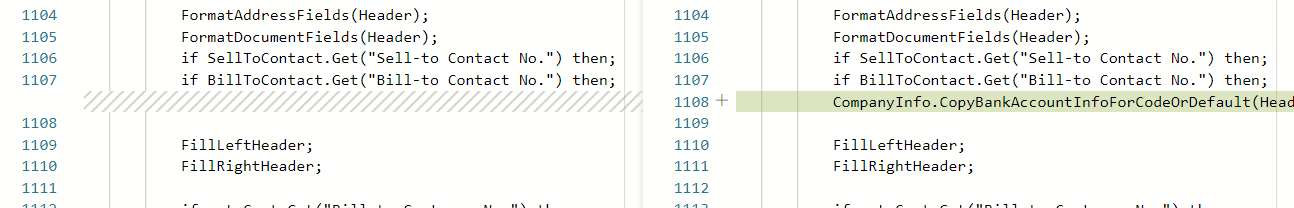
\includegraphics[width=\textwidth]{images/addinglinechange.png}
  \caption{Example of a change that added a line between what previously was line 1107 and 1108.}
  \label{fig:addinglinechange}
\end{figure}

\subsubsection{Removing lines from an AL object}
For removed lines, any test that was hitting what were previously those lines are selected.
\subsubsection{Adding an AL object}
We can not infer any test run from a new object, since coverage information would not include it.
\subsubsection{Removing an AL object}
We can see this case as being the same as removing all the lines of the object. Therefore any test hitting that object should be selected. It is worth noticing that this is not a traditional revision change, but it is taken into consideration for completeness.
\subsubsection{Adding lines to an AL test codeunit}
The current representation for the revision change does not distinguish if the lines added are because of adding new test cases on a given test codeunit, or because of changing a test procedure. Both cases could be treated differently if the model for the revision change allowed for that.

Instead, we only keep the information about which test codeunit lines were added. As a conservative approach, in this method, we select all test procedures inside this test codeunit.
\subsubsection{Removing lines from an AL test codeunit}
Similar to adding lines to an AL test codeunit, as a conservative measure, all tests in this test procedure are selected.
\subsubsection{Adding an AL test codeunit}
For this case, we select all the test procedures in the new test codeunit.
\subsubsection{Removing an AL test codeunit}
When the change is removing a test codeunit, we do not select any test case. However, the Object Id of the removed test codeunit is kept, to filter our selection by removing any references to such tests.
\subsection{The full algorithm}
We give an overview of how different parts of the selection method explained in the previous section compose together.

A codebase at a given point in time can be enriched when running the test suite with the information of the lines covered by each test case. This is achieved through the modifications on the \emph{Test Runner} application explained in section \ref{section:cov-info}. This information is stored in a coverage database.

When a revision is given, we know the set of file paths and lines changed. We can leverage from parsing such files on each revision to gather more information about what this revision change implies. The information extracted allows for different test selection criteria for each type of change, as it is listed in section \ref{section:rev-diffs}, table \ref{table:revision-changes}. In general, consider this step as extracting an expressive representation of the revision changes.

With this information, the test selection criteria described in section \ref{section:test-selection} is then applied, resulting to a set of selected test cases.

Figure \ref{fig:testselection} shows a diagram to further illustrate the above description.
\begin{figure}[H]
  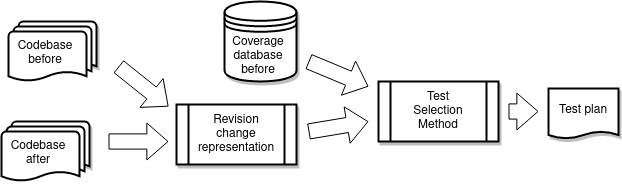
\includegraphics[width=\textwidth]{images/testselection.png}
  \caption{Diagram of the procedure for test selection.}
  \label{fig:testselection}
\end{figure}

\section{Evaluation}\label{section:evaluation}
\subsection{Metrics}\label{section:metrics}
In the literature for the problem of test selection, several metrics have been proposed to quantify the different aspects addressed by a selection algorithm.

For example, counting how many methods were selected, relates to the expected performance improvement when executing this reduced test suite. After all, choosing all tests is a valid selection algorithm, although not ideal for our goal.

Another example is measuring how effective the algorithm was to select the faulty test cases. If our selection is very small it would be efficient, but if such selection is not capturing the faulty tests, then it is damaging to the product quality.

We select metrics based on a survey done by Pan, Bagherzadeh, et. al. in \cite{Pan2021TestCS} on this topic. One of the research questions they dealt with, was the metrics used to evaluate the Test Selection and Prioritization (TSP) problem. Additionally, other common simple metrics were used, these were according to the metrics used by a similar approach from Beszédes et. al. \cite{6405252}.

\subsubsection{Test selection execution time}
This metric measures the total time of running the selected subset of tests, against the total time that it takes to run all of them.

Ideally, it is desirable for this value to be as small as possible.
\subsubsection{Test selection time to first failure}\label{section:tffailure}
This metric measures the time taken for test execution until the first failure is detected, according to the proposed plan; with respect to the total execution time of all tests. This is a metric for evaluating a test prioritization technique, since a selection may have different orderings, and each order would change the value of this metric.

In such context, we take the selection to be the prioritized set and take one of the orderings arbitrarily. This is a relevant metric to implement since in further work we aim to also evaluate prioritization techniques.

Ideally, it is desirable to detect failures as quickly as possible, that is, the time taken to run the test that fails the quickest.
\subsubsection{Inclusiveness}
This metric was first introduced by Rothermel and Harrold in \cite{Rothermel1997ASE}, and it refers to the ratio of the failing test cases included out of the total number of failing test cases. Therefore, for a test selection algorithm that includes all the failing test cases, we would aim to have a value close to 1 for this metric.
\subsubsection{Selection size}
For this metric, the ratio of the selected tests against the total amount of tests is taken. Ideally, we aim at as low number as possible while detecting every failing test case.
\subsubsection{Normalized APFD}
Average of the Percentage of Faults Detected is another commonly used metric to measure the effectiveness of Test Prioritization algorithms. First introduced by Rothermel et. al in \cite{962562}.

This metric measures the area under the curve of the plot of tests run against faults detected. The normalized version takes into account possibly not detecting faults, which is the case for a selection algorithm. For completeness, the expression for computing it is given in (\ref{eq:napfd}).

\begin{equation}
  \label{eq:napfd}
    nAPFD = p - \frac{\sum_{i=1}^{m}TF_i}{nm}+\frac{p}{2n}
\end{equation}
Where $p$ is the ratio of detected over total faults; $n$ is the total number of test cases; $m$ is the total number of faults, and $TF_i$ is the ranking of the first test case that revealed the fault of the $i$-th failure.

This value measures the proportion of area covered by the described plot, therefore it is desirable for this area to be as close to 1 as possible.

\subsection{Selecting real revision examples}\label{section:evaluation-real}
In this section, we describe the process and difficulties of providing examples of real revision changes that made a test fail. We also outline the required changes for future work. We present the metrics obtained from running the evaluation in a single failing revision example. While we are aware of the limitations to argue given these results, the main outcome was the engineering knowledge of the process to build a proper evaluation dataset.

The build system used for Business Central is referred to as DME. Roughly described, when a developer submits a test job, its branch gets built and tests get to run against it. After some time, the developer receives information on whether or not the changes can be integrated into the main branch for the product release being worked on.

A test job is composed of several interdepending tasks, and building the target system for which the tests are run is not a straightforward process. As an example, the codebase at a given point in time is a representation of several AL applications, each of which can be localized (country-specific logic organized within \emph{layers}). This means that running tests involves localizing the codebase for each country, building each application, building the appropriate databases, and executing different test solutions on it.

Trying to match this with the simple context we had so far analyzed, increased the complexity for running evaluations. However, the DME system is capable of being queried for further integrations, and in principle most of the process to get the evaluation point is possible, and to a certain degree can be automated.

For this project, a program was made to query and extract information about this system, to collect failing test jobs on real revisions.

The main complication that we faced was getting a reproducible revision example, together with the long time that these heavy operations take, as they are usually performed on clusters of machines for this purpose.

Nevertheless, we present the case of job 2412636, a case where we were able to extract the line coverage information and get a prediction with the test selection method proposed. In this test job, changes to an extension \texttt{INTaxEngine} were made. The corresponding test extension where failures were found is \texttt{TaxEngine-JsonExchange}. After obtaining the codebase for such revisions, the database and views were constructed for the failing version. In this case, the localized version corresponds to the Indian version. To this setup, the modification to the test runner was applied, and the test suite was run again on both revisions, collecting the coverage information for the initial revision.

Afterward, the test selection algorithm was executed. Figure \ref{fig:evalalgout} shows the output of the selection algorithm and figure \ref{fig:evalfailures} the failures that occurred in the build system. We can observe that for this case, the inclusiveness results in 0. No selected test was failing. When looking at the stack trace of the error, we can see that the failure was due to not having permissions on new tables after their modifications. These types of faults are hard for our current algorithm to tackle since they depend on the context that the revision introduced. This is not corresponding directly to statements or lines on the codebase, and therefore only using line coverage information does not suffice. In the next section, when evaluating against injected faults on the system, a class for the proposed changes made is context-faults that resemble faults like the ones detected for this job.


\begin{figure}[H]
\begin{verbatim}
136802 TestInitializeTaxRates
136802 TestUpdateTaxRates
136802 TestUpdateFromAndToRangeAttributeOnTaxRates
136802 TestUpdateLinkdAttributeOnTaxRates
136802 TestUpdateFromAndToRangeAttributeForError 
\end{verbatim}
\caption{Output of the Selection algorithm for job 2412636.}
\label{fig:evalalgout}
\end{figure}

\begin{figure}[H]
\begin{verbatim}
137700 TestImportTaxTypes
137700 TestExportTaxTypes
137700 TestExportNodes
137700 TestUseCaseExecution
137700 TestUseCasePosting
137700 TestTaxInformationFactbox
137700 TestUseCasePostingExecution
\end{verbatim}
\caption{Failing tests on job 2412636.}
\label{fig:evalfailures}
\end{figure}

The program built for querying the build system provided different failing test jobs together with the log files associated with them. We could use them as starting point to collect the required information and attempt to reproduce them. However, we faced difficulties in streamlining this process. We list some of them.

The failing job could be dismissed if the job was submitted as a private deployment for the developer, since developers can request jobs from the pipeline without publishing their changes to the remote repository, making it inaccessible for us to obtain.

If the pull request associated with the test job was closed, typically the branch gets deleted as well, making it impossible to get the commit where the failing job was executed.

Also when obtaining the database and binaries associated with the build version, typically only the latest are provided to the developers since those are the ones required for their work. But to reproduce some of the job errors, it required in some cases to change the version of the binaries used. Overall, this made the process prone to failure and it needed a large investment of time.

In future work, we aim to integrate the collection of evaluation information on the CI pipeline, so that reproducibility errors are not an issue. With these changes, we could use the existing build system and resources to produce the required information at the time of failure. To do this, changes would be required on the build system, which themselves live under the main application repository in the form of Infrastructure-as-Code. We expand more on this in section \ref{section:future-work}.

\subsection{Injecting faults in the codebase}
Given the challenges concerning reproducing real examples of code changes and the corresponding test failures within this project's timeline, we use fault injection to build a set of examples for evaluation. Modifications were purposefully made to make part of the tests fail. We did this however to state that we are capable of computing and gather some insight on the results of this selection.

We used two test extensions from the real application: \texttt{Bank} (Test cases 1-4) with 454 test procedures and \texttt{VATGroupManagement} (Test cases 5-8) with 75 test procedures. 

We can identify some classes of the mutations made, based on the type of modifications. However, we do not argue that they are representing the full set of the actual test failures that the system usually experiences. 

Depending on how lines are mapped to statements we classify the kinds of bugs introduced as follows:

\begin{itemize}
\item Context-fault. Lines changed for this kind of bugs did not correspond to statements on the execution, but in the side-effects they produced. Test cases \#3, \#4, \#7, and \#8 belong to this class.
\item Statement-fault. Lines changed correspond to statements on a sequential procedure and therefore are easily captured by the heuristic we used. 
\end{itemize}

\begin{table}[H]
\centering
\begin{tabular}{||l|l|l|l|l|l|l||}
\hline
Test case& Type&$t_{Full} (\%)$ & $t_{FF} (\%)$ & $i$ & $size (\%)$ & $nAPFD$ \\ \hline\hline
\#1&Statement&60.028 & 0.044 & 24.615 & 34.549 & 20.004\\
\#2&Statement&0.058 & 0.027 & 100 & 0.796 & 99.867 \\
\#3&Context&71.006 & NA & 0 & 44.562 & 0\\
\#4&Context&84.198 & NA & 0 & 49.337 & 0 \\
\#5&Statement&35.402 & 17.968 & 100 & 21.212 & 87.121 \\
\#6&Statement&33.216 & 33.216 & 100 & 21.212 & 79.545 \\
\#7&Context&0 & NA & 0 & 0 & 0 \\
\#8&Context&37.058 & NA & 0 & 24.242 & 0 \\
\hline
\end{tabular}
\caption{Evaluation of injected faults.}
\label{table:evaluation}
\end{table}

In the previous table, $t_{Full}$ refers to the percentage of time taken to execute the complete selection, $t_{FF}$ is the percentage of time until the first failure was detected, $i$ is the inclusiveness, $size$ and $nAPFD$ are given as a percentage (See section \ref{section:metrics}).

The results in table \ref{table:evaluation} show some of the insight we had previously discussed. When changing lines from a sequential procedure, the coverage information is useful and inclusiveness is significant. However, when changes related to the context were made, the inclusiveness was zero.

For example, one of the faults changed the visibility of the fields of a page. After this, a UX test scenario failed. However, a common pattern for these situations in AL is for the visibility to not be controlled directly by statements on procedures, but by a globally controlled boolean that sets the \texttt{Visible} property of the field. Therefore, since changes did not correspond to statements, this selection did not include the failing tests.

In another case, no test had coverage information for the lines changed, and the selection was empty.

It is also relevant to note that the size of some of these selections was considerably large. For example, in cases \#3 and \#4, nearly half of the test cases were selected, but none of those were the faulty ones. Observing the time of fully executing for case \#4 shows it was 84.198\%. A possible explanation for the large size is that some test cases have a large density of lines covered. This is the case of tests in the \texttt{Bank} extension, where the test case that covers most lines covers 10285 lines, and the average of lines covered is 4191.90. In contrast to tests in the \texttt{VATGroupManagement} extension with maximum lines covered 1778 and an average of 365.64.

\section{Related work}\label{section:alg-and-context}

In this section we expand on the comparison with methods found in literature, to also outline possible directions for future work. As a starting point, two related surveys are used: one by Yoo and Harman \cite{Yoo2009RegressionTM} for general minimization, selection, and prioritization techniques, to put in perspective the current approach with the academic context. And the work by Pan, et. al in \cite{Pan2021TestCS} where they focus on techniques using Machine Learning, to understand what inputs are required to understand how applicable these techniques can be in future work.

The implemented technique here follows quite precisely the formulation for identifying fault-revealing test cases given by Rothermel and Harrold in \cite{Rothermel1997ASE}. Here they define a modification-traversing test as a test with different execution traces for two given revisions of a codebase. Such tests can happen when either they execute new or modified code in the new revision, or if they formerly executed code deleted in the new revision.

By using the \emph{Controlled-Regression-Testing Assumption} they can prove that modification-traversing selected test cases are a superset of the possible fault-revealing test cases. This is a strong assumption, and in our case it does not hold, as we gave insight for in section \ref{section:overview}. There are faults that test cases reveal that are context-aware, they do not correspond to the execution traces of the test cases. For instance, the real evaluation example described in section \ref{section:evaluation}.

The algorithm they propose \emph{SelectTests} compares Control Flow Graphs (CFG) generated from each test case, and when different, select all the tests that reached such nodes. Our approach can be considered a loose approximation of this, but we do not rely on generating a CFG for the execution of the new revision of test cases, but we directly interpret line operations on files as a difference and select the corresponding cases. We differ on how we decide whether or not execution traces of a test are equivalent.

Work and terminology introduced by Rothermel and Harrold \cite{Rothermel1997ASE} were foundational for the area and it has been used as a framework to communicate results in surveys and other papers. That is the case of another similar approach by Vokolos and Frankl\cite{Vokolos97pythia}, similar to this project, they also take \texttt{diff} information as input for their selection; in the same fashion, they characterize each line operation, and associate a set of tests depending on the execution traces from previous revisions. The main difference is the preprocessing of revisions into a normal form to have a better correspondence between lines and execution traces. This is a direction that could be interesting to explore to increase the precision of selected test cases.

The similarity between the CFG traversing approach of Rothermel and Harrold with the textual difference approach from Volkolos and Frankl was hinted at when we compared how similar our approach was with the CFG approach. This was also observed by Yoo and Harman on their survey, noticing that the textual approach operated on a different representation of the system, but the behavior was in essence very similar.

Another related approach that could hint a direction on an extension of the technique proposed here is the work by Chen et. al. \cite{chen} where the CFG is extended by changing the definition of how a program can be partitioned. Changing this representation allows for more entities to be considered. Extending the representation of AL files, and giving a way to relate coverage information with different representations could allow more information to be captured, increasing the inclusiveness of our approach.

A very similar approach was also found in \cite{6405252} by Beszédes et. al., where they describe the implementation of a coverage-based selection technique on the C++ components of the WebKit project. They follow a similar approach in the technical perspective, by implementing a procedure-level coverage database instead of a line coverage database. They identify changed modules from a revision change and execute the related test cases according to their coverage database. This is an analogous process to the one we follow, only taking a coarser perspective by grouping the different changes on the procedures it affected.

On the other hand, a more recent survey focuses on the techniques using Machine Learning algorithms \cite{Pan2021TestCS}, as they have been the subject of much interest in recent years. Rather than comparing them with the proposed selection algorithm, we present some of the applicable techniques that were found, for the focus of future work.

Conveniently, the survey exhibits a classification of the methods by artifacts and information provided by the papers\cite{MAHDIEH2020106269}\cite{10.1109/ICSE.2019.00055}\cite{10.1145/3180155.3180210}. This can be very useful if we want to compare different selection criteria with the tools provided by the authors, adapting the collected information to their required inputs. We elaborate on the techniques found.

The technique proposed by Mahdieh, et. al. in \cite{MAHDIEH2020106269} uses a neural network after extracting a set of features from the codebase. These features consist of different metrics for the faulty revision, for instance, complexity metrics, coupling metrics, documentation metrics, or inheritance metrics defined for Java programs. It also uses the code coverage grouping by procedure as the approach from Beszédes et. al. described above. Such features are then the input of a neural network binary classifier that predicts whether or not a test case will be a fault-revealing one. In this technique, code coverage is used for prioritization.

The family of techniques presented by Cruciani et. al. in \cite{10.1109/ICSE.2019.00055} and \cite{10.1145/3180155.3180210} take a different approach, by noticing that TSP is a big data problem and proposing techniques based on similarity. The main benefit of these approaches is that the core procedure in which they are based does not require any information but the test cases themselves. They use a vector space representation for each test and use clustering algorithms to determine which tests cases to use. This makes them highly scalable. The input of the tool provided is this vector space representation of the test cases. We could adapt generating such representation from AL test cases, as the features required rely on textual information and randomized projections.

\section{Future work}\label{section:future-work}
Throughout this report, we have hinted at possible directions for future work. In this section, we summarize and expand on them. 

\subsection{Different revision representations}
Among the different techniques that were shown to be similar in section \ref{section:alg-and-context}, a missing step on the current implemented technique was getting more information about the changes made in the codebase. For example, in \cite{6405252} they identify the procedures where the changes were made by using different source code representation tools. Also in \cite{962562}, they depend on using a CFG representation of the tests, to match such information and identify in which node of the graph were changes made.

A future direction can be extracting more semantical information from a given change. AL compiles into C\# code, which is used by the runtime server of the application to execute the required business logic. C\# is a widely studied language with several source code representation tools that we can leverage.

This is also relevant to explore Machine Learning techniques since a common step for most of these techniques is feature extraction. This consists of extracting more information, from the source code, coverage information, and historical information about the test cases.

\subsection{Applicable techniques from the literature}
In section \ref{section:alg-and-context}, we went over the different existing approaches to regression testing that followed similar ideas to the one proposed here. Some of the insight collected from such implementation can aid our algorithm and could be a way for extending it, like preprocessing files into a normal form or having different representations for AL files.

We also listed some applicable ML techniques\cite{MAHDIEH2020106269}\cite{10.1109/ICSE.2019.00055}\cite{10.1145/3180155.3180210}, that use the information we have available, or for which some changes are required. Those are the family of FAST techniques from Cruciani et. a.l. \cite{10.1109/ICSE.2019.00055} and the neural network approach of Mahdieh, et. al. \cite{MAHDIEH2020106269} our aim is to compare and extend the technique proposed in this project with their provided artifacts.

\subsection{Infrastructure for integrating evaluation on CI/CD pipeline}
To increase our confidence in the validity of the results, we need a more robust evaluation method. For this project, we obtained manually the revision information of existing failing jobs and re-executed the test job failures collecting the coverage information to have the required inputs for our selection algorithm. This process was shown to be hard to reproduce, as explained in section \ref{section:evaluation-real}.

A better approach to this problem would be not to reproduce the error as it happened while collecting the required information. Instead, to collect that information from the job itself. This would require changes in the infrastructure pipeline.

The pipeline and plan executed by the build system are kept in the same repository as Infrastructure-as-Code. Modifications would result in executing different tasks, like the collection of the coverage information.
 The scope of future work here should focus on making modifications to these task execution models for evaluation data collection.

\subsection{Efficiency of producing coverage database}
A relevant engineering concern not addressed when introducing the proposed coverage database is the efficiency of producing the coverage database. While having a database allows for more efficient and flexible querying of information instead of the existing CSV schema of processing coverage; it comes currently with a toll in performance when populating the coverage database.

There are several optimizations possible regarding transaction management in SQLite and other configuration options for the engine like using prepared statements. This work item becomes increasingly important if looking to integrate the evaluation on the CI/CD pipeline since it should not be considerably more expensive to obtain such a database than the current process for collecting coverage information.

\subsection{Other evaluation metrics}
Related to the previous item, other metrics would give better insights to understand how likely would it be to adopt the techniques on the real system. As observed in \cite{10.1109/ICSE.2019.00055}, test selection is a process with several phases, following the literature these phases are: an analysis phase, an execution phase, and a collection phase. The current metrics only deal with the execution phase of the algorithm, however, the cost of collecting the coverage information currently is significant. Only measuring one of the phases skews the evaluation of how adoptable is this approach.

\section{Conclusion}

Throughout this project, we built some parts of the required infrastructure to run test selection techniques on real revision examples of Business Central. We also implemented a basic selection technique. There still exists a difficulty in streamlining the evaluation of real revision examples, however, we have given an outline of the required changes to increase the validity of our evaluation in future work. This would increase the dataset, and provide the required information for real test failures in the build system without the need of reproducing the failures.

We have obtained insights on the current limitations of the approach with the limited evaluation dataset built from injecting faults into the real system. One insight is the difficulty of selecting faulty test cases when the changes are on the side-effects rather than on sequential statement execution. Also, the large selection proposed by this approach when test cases cover a large number of lines.

We also located the approach in its context and qualitatively compared them with other approaches. Such comparisons led to ideas that could be used to extend the selection algorithm in future work. After this, we also evaluated techniques using Machine Learning that have artifacts available and require input information that we could obtain. \footnote{Artifacts for this project can be found in \href{https://github.com/mynjj/research-project-itu}{https://github.com/mynjj/research-project-itu}}



\begin{thebibliography}{10}

\bibitem{Pan2021TestCS}
  Rong Pan and Mojtaba Bagherzadeh and Taher Ahmed Ghaleb and Lionel C. Briand,
  \textit{Test Case Selection and Prioritization Using Machine Learning: A Systematic Literature Review},
  ArXiv, 2021, abs/2106.13891

\bibitem{Yoo2009RegressionTM}
  Shin Yoo and Mark Harman,
  \textit{Regression Testing Minimisation, Selection and Prioritisation - A Survey},
  2009

\bibitem{Rothermel1997ASE}
  Gregg Rothermel and Mary Jean Harrold,
  \textit{A safe, efficient regression test selection technique},
  ACM Trans. Softw. Eng. Methodol., 1997, volume=6, pages=173-210
}

\bibitem{962562}
  Rothermel, G. and Untch, R.H. and Chengyun Chu and Harrold, M.J.,
  \textit{Prioritizing test cases for regression testing},
  IEEE Transactions on Software Engineering, 2001, volume 27 number 10 pages 929-948,10.1109/32.962562

\bibitem{6405252}
  Beszédes, Árpád and Gergely, Tamás and Schrettner, Lajos and Jász, Judit and Langó, László and Gyimóthy, Tibor,
  \textit{Code coverage-based regression test selection and prioritization in WebKit},
  2012 28th IEEE International Conference on Software Maintenance (ICSM), 2012, 10.1109/ICSM.2012.6405252

\bibitem{MAHDIEH2020106269}
  Mostafa Mahdieh and Seyed-Hassan Mirian-Hosseinabadi and Khashayar Etemadi and Ali Nosrati and Sajad Jalali,
  \textit{Incorporating fault-proneness estimations into coverage-based test case prioritization methods},
  Information and Software Technology, 2020, https://doi.org/10.1016/j.infsof.2020.106269

\bibitem{10.1109/ICSE.2019.00055}
  Cruciani, Emilio and Miranda, Breno and Verdecchia, Roberto and Bertolino, Antonia,
  \textit{Scalable Approaches for Test Suite Reduction},
  IEEE Press, Proceedings of the 41st International Conference on Software Engineering, 2019, pages 419-429, 10.1109/ICSE.2019.00055

\bibitem{10.1145/3180155.3180210}
  Miranda, Breno and Cruciani, Emilio and Verdecchia, Roberto and Bertolino, Antonia,
  \textit{FAST Approaches to Scalable Similarity-Based Test Case Prioritization},
  Proceedings of the 40th International Conference on Software Engineering, 2018, pages 222-232, 10.1145/3180155.3180210
\bibitem{chen}
  Chen YF, Rosenblum D, Vo KP.
  \textit{Testtube: A system for selective regression testing},
  Proveedings of the 16th International Conference on Software Engineering (ICSE 1994), ACM PressM, 1994; 211–220.
\bibitem{Vokolos97pythia}
    F. I. Vokolos and P. G. Frankl,
    \textit{Pythia: A regression test selection tool based on textual differencing},
    1997
}

\end{thebibliography}


\end{document}
